\chapter{提案手法} \label{chap:algorithm}
本章では提案手法を詳しく説明する.
まず,\secref{flow}にて自動生成の大まかな流れを説明し,その後にそれぞれの工程について詳しく述べる.
\secref{input}および\secref{output}にて入出力について説明し,
\secref{device}にて使用するデバイス,
\secref{software}にて使用するソフトウェア,
\secref{3Dmodel}にて使用する3Dモデルについて述べる.
\secref{analysis}にてMIDIデータの解析からモーションへの適用方法を説明する.
そして最後に,\secref{howto}にて実際にシステムを使用する際の,使用方法について言及する.

\section{自動生成の流れ} \label{sec:flow}
\figref{fig:flow}に,音源から吹奏アニメーションを自動生成する流れを示す.\\
\begin{figure}[h]
	\centering
	\includegraphics[width=14cm]{fig/chap3/flow.eps}
	\caption{音源から吹奏アニメーションを自動生成する流れ}
	\label{fig:flow}
\end{figure}
\indent
実際のアニメーション制作フローに沿わせるため,音源の生成は楽器を用いて行う.
次に,生成した音源を解析し,譜面データへ変換する.
そして,アニメーション生成と同時に音源を流すことにより,音源に合わせてキャラクタが動くアニメーションが完成となる.

\section{入力} \label{sec:input}
入力する音源は,MIDI音源とする.
ここで,MIDI音源は,MIDIという信号を受信して発音する音源のことである.
よく使用されるmp3やwaveなどの形式とは異なり,中身が譜面データとなっているため,音の解析が比較的容易である.\\
\indent
このMIDI音源を生成する方法は,後述する.

\section{出力} \label{sec:output}
出力は,管楽器を演奏するキャラクタのアニメーションである.
今回対象とする管楽器は,トランペット,トロンボーンである.
この2本の楽器を選んだ理由は,吹奏楽ではとくに目立つ楽器であり,3Dモデルが入手しやすかったために選んだ.

\section{デバイス} \label{sec:device}
MIDI音源を生成するために,電子楽器であるウインドシンセサイザ「EWI5000」(\figref{fig:ewi})を使用する.
このウインドシンセサイザは,さまざまな楽器の音を再現することが可能である.
\begin{figure}[h]
	\centering
	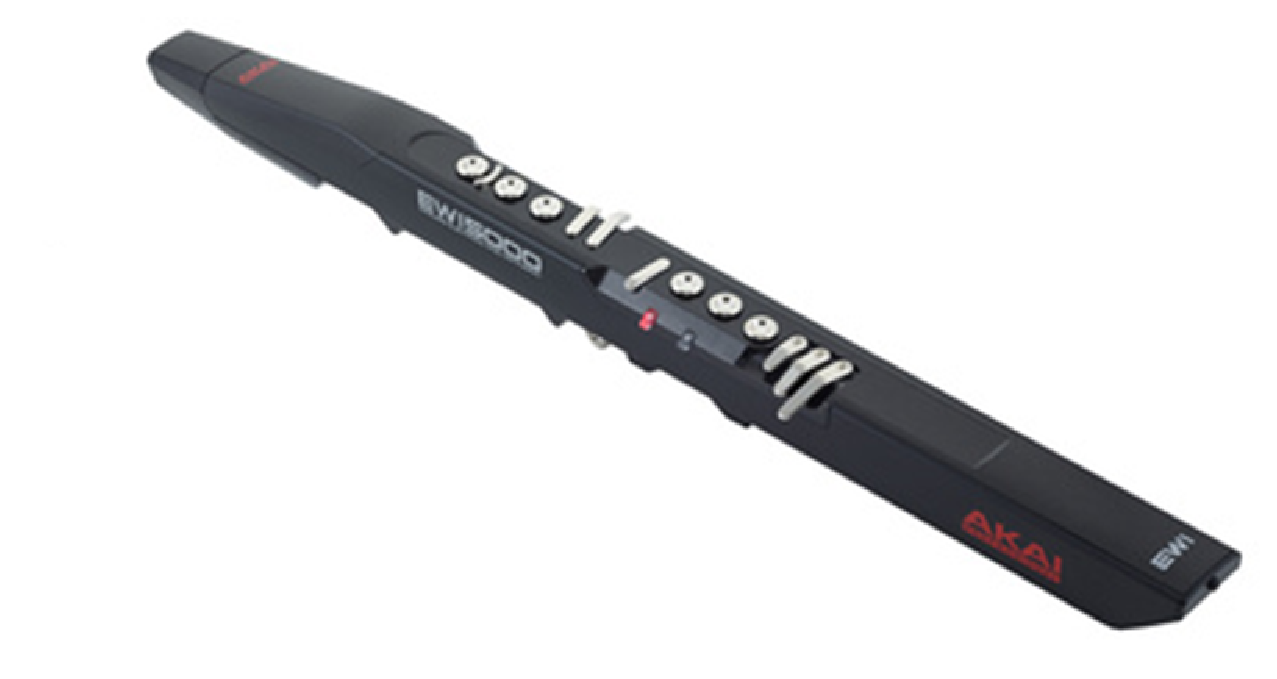
\includegraphics[width=10cm]{fig/chap3/ewi.eps}
	\caption{ウインドシンセサイザ「EWI5000」}
	\label{fig:ewi}
\end{figure}

\section{ソフトウェア} \label{sec:software}
\secref{device}で述べたウインドシンセサイザは,単音しか鳴らすことができないため,シングルチャンネルの音源しか生成することができない.
しかし,吹奏アニメーションを自動生成するためには,複数人で演奏しているマルチチャンネルの音源が必要となる.
そこで,ウインドシンセサイザで生成したMIDI音源を,フリーソフトウェアであるMIDIシーケンスソフトウェア「Domino」(\figref{domino})に出力し,重ねて何度も録音することにより,マルチチャンネルの音源を生成する.
\begin{figure}[h]
	\centering
	\includegraphics[width=10cm]{fig/chap3/domino.eps}
	\caption{MIDIシーケンスソフトウェア「domino」}
	\label{fig:domino}
	
\end{figure}

\section{3Dモデル} \label{sec:3Dmodel}

\section{MIDIデータの解析} \label{sec:analysis}

\subsection{楽譜データへの変換}

\subsection{モーションへの適用}

\section{本システムの使用方法} \label{sec:howto}